%!TEX root = ./main.tex
\section{Background}
\label{sec:bg}

\subsection{Defination of resugaring}
This subsection is partially similiar to original defination in\cite{resugaring}.
\begin{Def}[Resugaring]
Given core language (named {\bfseries CoreLang}) and its evalation rules, together with surface language based on syntactic sugars of CoreLang (named {\bfseries Surflang}). For any expression of Surflang, getting the evaluation sequences of the expression in terms of SurfLang. 
\end{Def}
For correctness of the resugaring, the evaluation sequences should maintain the following three properties:
\begin{enumerate}
\item {\bfseries Emulation} The evaluation sequences reflect the actual execution process.
\item {\bfseries Abstraction} The resugaring sequences should only contains terms in SurfLang, and each term of SurfLang should originate from initial expression.
\item {\bfseries Coverage} No sequence is skipped during the process.
\end{enumerate}

Given an example below.

For syntactic sugar {\bfseries and} and {\bfseries or}, the sugar rules are:
\begin{center}
	\parbox[t]{\textwidth}{%
		\begin{center}  
			and(e1, e2) → if(e1, e2, \#f)\\
			or(e1, e2) → if(e1, \#t, e2)
		\end{center}  
	}%  
\end{center}
which forms a simple SurfLang.

The evaluation rules of {\bfseries if} is:
\begin{center}
	\parbox[t]{\textwidth}{%
		\begin{center}  
			if(\#t, e1, e2) → e1\\
			if(\#f, e1, e2) → e2
		\end{center}  
	}% 
\end{center}

Then for SurfLang's expression $\mbox{and}(\mbox{or}(\#f, \#t), \mbox{and}(\#t, \#f))$ should get resugaring sequences as fig\ref{fig:example}.

\begin{figure}[ht]
\parbox[t]{\textwidth}{
			\begin{center}  
				(and (or \#f \#t) (and \#t \#f))\\
				↓\\
				(and \#t (and \#t \#f))\\
				↓\\
				(and\#t \#f)\\
				↓\\
				\#f
			\end{center}  
		}
\caption{resugaring example}
\label{fig:example}
\end{figure}

The reason we should get the sequences above is because $(\mbox{and}~(\mbox{or}~\#f~\#t)~(\mbox{and}~\#t~\#f))$ should desugar to $(\mbox{if}~(\mbox{if}~\#f~\#t~\#f)~(\mbox{if}~\#t~\#f~\#f)~\#f)$. Then in the CoreLang, the evaluation sequences will be as fig\ref{fig:coreseq}.

\begin{figure}[ht]
\parbox[t]{\textwidth}{
			\begin{center}  
				(if (if \#f \#t \#f) (if \#t \#f \#f) \#f)\\
				↓\\
				(if \#t (if \#t \#f \#f) \#f)\\
				↓\\
				(if \#t \#f \#f)\\
				↓\\
				\#f
			\end{center}  
		}
\caption{evaluation sequences}
\label{fig:coreseq}
\end{figure}

The second item in the sequences can be desugared from $(\mbox{and}~\#t~(\mbox{and}~\#t~\#f))$, so resugars to it. So as the third item.

\subsection{Background}
{\bfseries Church–Rosser theorem}\cite{churchrosser} gives theoretical support for full-$\beta$ reduction, which is a nondeterministic evaluation strategy of lambda caculus. 

{\bfseries Reduction semantics}\cite{reduction} is an alternate presentation of structured operational semantics\cite{PLOTKIN}. The difference is that it use context rules uniquely to restrict evaluation order, instead of hidden in inference rules. The holes (E) in the context rules is where reductions can take place.

\begin{figure}[ht]
	\centering
	\[\infer {(v~e) \rightarrow (v~e')}{e~\rightarrow~e'}  \]
	\[\infer {(e~e'') \rightarrow (e'~e'')} {e~\rightarrow~e'}  \]
	\caption{Plotkin's lambda}
	\label{fig:plotkin}
\end{figure} 

\begin{figure}[ht]
	\centering 
	E = (E e) | (v E) | []
	
	if e $\rightarrow$ e' then E[e] $\rightarrow$ E[e']
	\caption{Reduction semantic}
	\label{fig:felleisen}
\end{figure} 

Our original idea is similiar to full-$\beta$ reduction. When not restricting the context rules of reduction semantics, the reduction paths of a expression will become a full graph like full-$\beta$ reduction. For the $\mbox{and}(\mbox{or}(\#f, \#t), \mbox{and}(\#t, \#f))$ example, we allow all expressions reducible. Then we can get the following full reduction graph as Fig\ref{fig:fullreduction}.

\begin{figure}[ht]
	\centering
	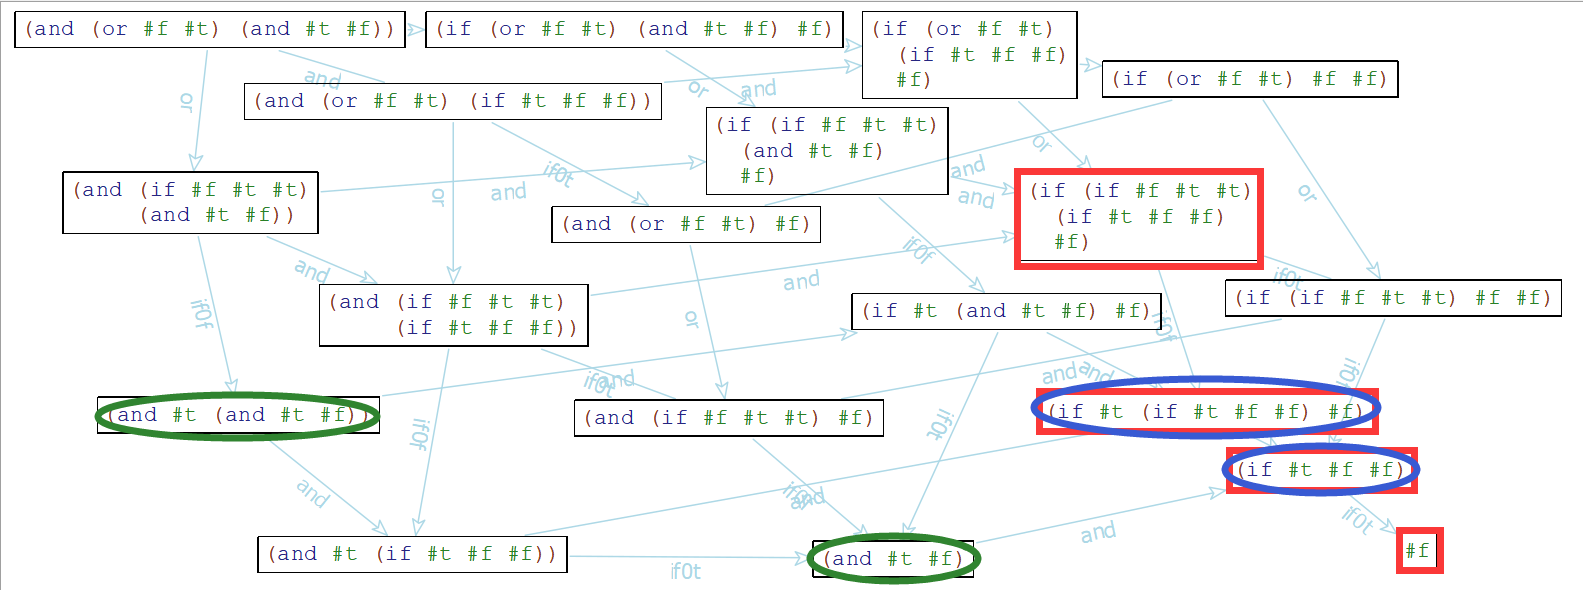
\includegraphics[width=12cm]{images/fullreduction.png}
	\caption{full reduction's example}
	\label{fig:fullreduction}
\end{figure}

We could find that the subsequences marked by red are the evaluation sequences after the syntactic sugar expression desugared. The subsequences marked by blue are which can be resugared. The subsequences marked by green are the resugaring sequences we want to get.

(zc's approach)

In this paper, we use reduction semantics as theoretical basis. PLT Redex is a semantic engineering tool based on reduction semantics. We use the tool for implementing our approaches.

